\documentclass[10pt]{article}

\usepackage{titlesec}
\usepackage[singlespacing]{setspace}
\usepackage[letterpaper,margin=0.75in]{geometry}

\setcounter{tocdepth}{4}


\usepackage{hyperref}
\usepackage{geometry}
\usepackage{graphicx}
\usepackage{float}

\usepackage{lastpage}
\usepackage{fancyhdr}
\fancyfoot[C]{Page \thepage\ of \pageref{LastPage}}

\usepackage{listings}
\usepackage{color}
 
\definecolor{codegreen}{rgb}{0,0.6,0}
\definecolor{codegray}{rgb}{0.5,0.5,0.5}
\definecolor{codepurple}{rgb}{0.58,0,0.82}
\definecolor{backcolour}{rgb}{0.95,0.95,0.92}
 
\lstdefinestyle{mystyle}{
    backgroundcolor=\color{backcolour},   
    commentstyle=\color{codegreen},
    keywordstyle=\color{magenta},
    numberstyle=\tiny\color{codegray},
    stringstyle=\color{codepurple},
    basicstyle=\footnotesize,
    breakatwhitespace=false,         
    breaklines=true,                 
    captionpos=b,                    
    keepspaces=true,                 
    numbers=left,                    
    numbersep=5pt,                  
    showspaces=false,                
    showstringspaces=false,
    showtabs=false,                  
    tabsize=2
}
 
\lstset{style=mystyle}

\begin{document}
\pagenumbering{gobble}
\begin{titlepage}
    \title{Guide Document}
    \author{Yeongae Lee, Jaehyung You \\ CS 463  \\ Oregon State University \\ Spring 2019 \\ \\ Project Physics Virtual Classroom: AsyncSync (Group 51) \\by Physics Department \\Dr. Kenneth Walsh}
    \date {June 10, 2019}

    \maketitle
        \begin{center}
           This document includes:\\
            Requirements \\
            Installation guide \\
            Backup guide \\
            User manual\\
            Additional information
        \end{center}     
\end{titlepage}

\section{Project Documentation}
    \subsection{Installation}
        \subsubsection{Prerequisite}
            You must be able to access the repository or the code. We are using Drupal8 as our developing environment. Any requirement will be installed if you follow the installation below. Any other requirement for using Drupal8, refer to the following link: https://www.drupal.org/docs/8/system-requirements
        
            \medskip \medskip \medskip
            \textbf{Note (You have to read this note before doing further actions):}
            \begin{itemize}
                \item The whole code for the current project is under "html" folder.
                \item You must use 'sqlbackup.sql' database file for completing to build the whole website. 
                \item Documents folder is for all the documentation of the project.
                \item ph-virtual-classroom is the code we worked on. Now, we don't use the code anymore.
                \item The code in this repository only gives you make a simple drupal website. (in 'html' folder)
                \item The site can't do any functions without the current server-database. (`sqlbackup.sql.zip')
            \end{itemize} 

        \subsubsection{Basic Program Installation: Drupal and MAMP}
            You may need to download Drupal8 (if the method I introduce below doesn't work) Drupal8 Download Clone git repository first. Please follow the following instructions (YouTube videos). You don't need to download Drupal from the Drupal website. You will use the  `html' folder as Drupal installer in this repository.
                \begin{itemize}
                    \item Install Drupal on MacOS: https://www.youtube.com/watch?v=pOBArJn-tSQ
                    \item Install Drupal on Ubuntu18.04: https://www.youtube.com/watch?v=9SEpG0rOs1w
                    \item Install Drupal on Windows: https://www.youtube.com/watch?v=4Gl9s40vldY
                \end{itemize}
            Our current server is running on Ubuntu. This guide does not include the guide for Linux users, so you may need to know how you can access `MyphpAdmin’ (We need this later) in your own Linux. \\
            \textbf{For Windows and MacOS users need to download `MAMP’ application to run the server. Download MAMP: https://www.mamp.info/en/downloads/}
           
        \subsubsection{Install Drupal and import Database on your local machine} 
            \begin{enumerate}
                \item Download MAMP and run MAMP. Then, you should see this program. Then, Click the `Start Servers’. The server is starting now.

                    \begin{figure}[!ht]
                        \centering
                        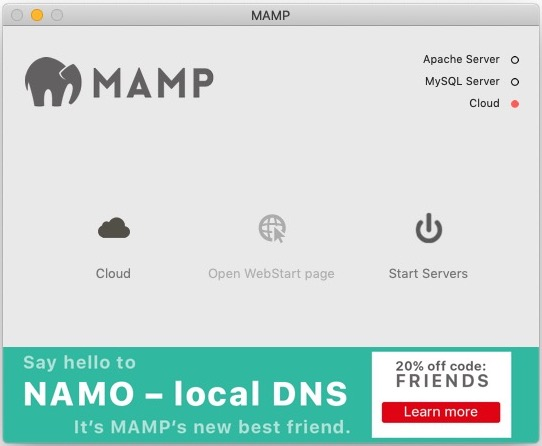
\includegraphics[width=0.35\textwidth]{Project_Document/MAMP}
                        \caption{MAMP Application}
                    \end{figure}
\newpage            
                \item Now you can see this page, then your MAMP application works. 
           
                    \begin{figure}[!ht]
                        \centering
                        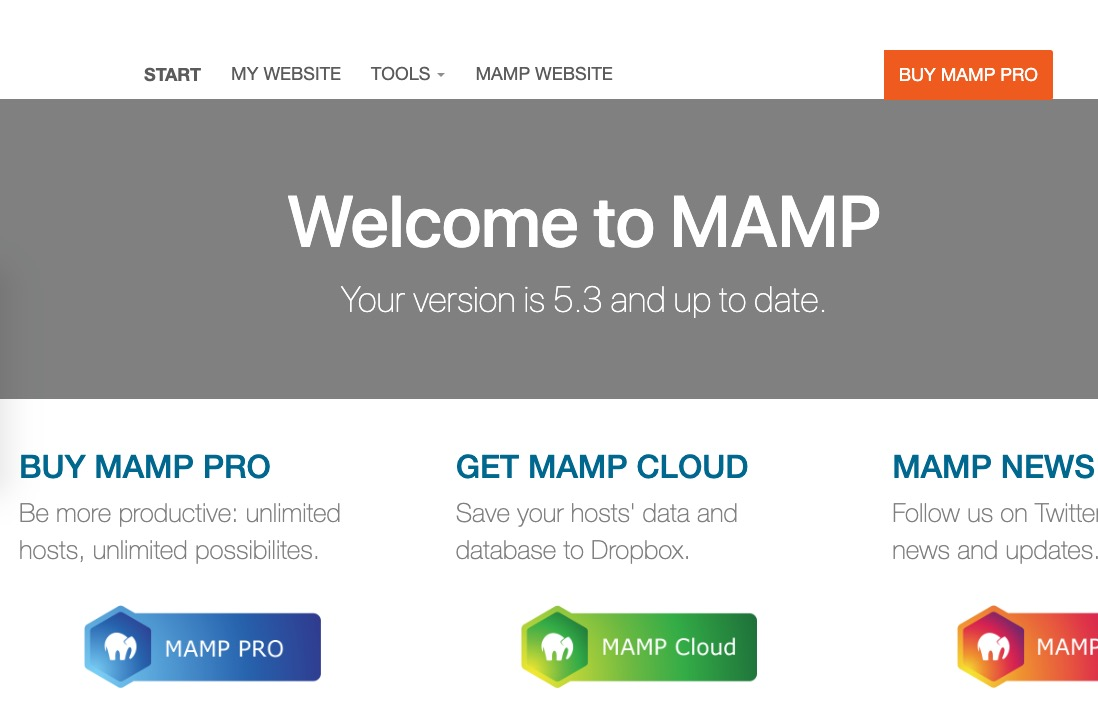
\includegraphics[width=0.55\textwidth]{Project_Document/setup}
                        \caption{MAMP Page}
                    \end{figure}      
            
                \item Now, you need to find the folder that will render your code to its server.

                    \begin{itemize}
                        \item For MacOS, move`html' from this repository to `/Application/MAMP/htdocs' (if you are using MAMP).
                        \item For Windows, move `html' from this repository to `Local Disk/MAMP/htdocs' (if you are using MAMP), and keep following the instruction for MacOS.
                        \item (if) For Ubuntu, locate to the folder `html' in /var/www/ (if you followed the instruction the above). 
                    \end{itemize}

                    \begin{figure}[!ht]
                           \centering
                           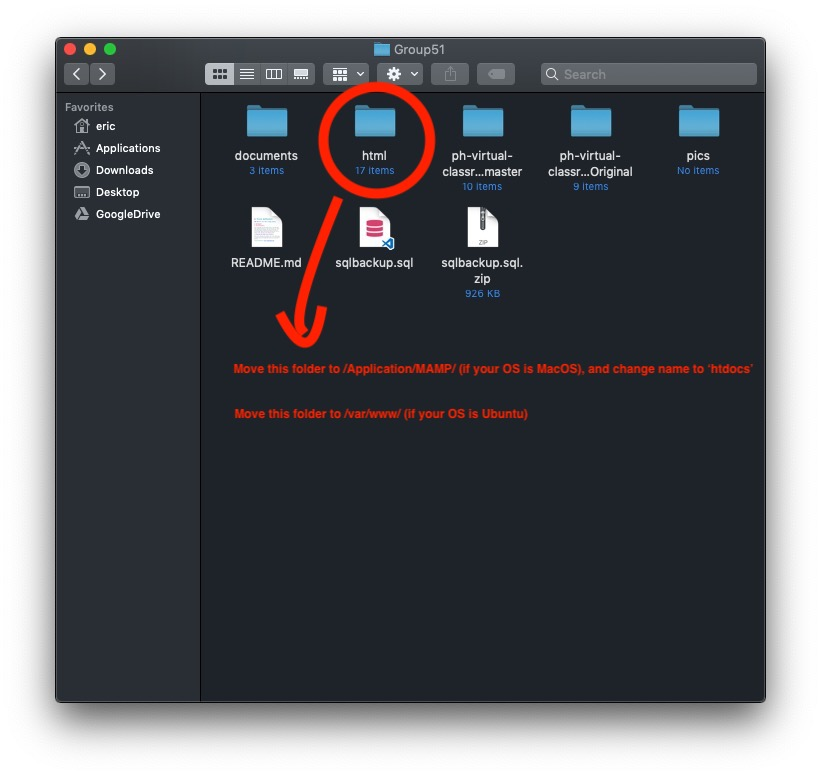
\includegraphics[width=0.7\textwidth]{Project_Document/macos}
                        \caption{Project File Folder}
                    \end{figure}  
\newpage                    
                \item You need to go to your `PHPMYADMIN’. This is where you can find `phpMyAdmin' by using MAMP (Click `TOOLS' in the banner, then click `PHPMYADMIN')
 
                    \begin{figure}[!ht]
                           \centering
                             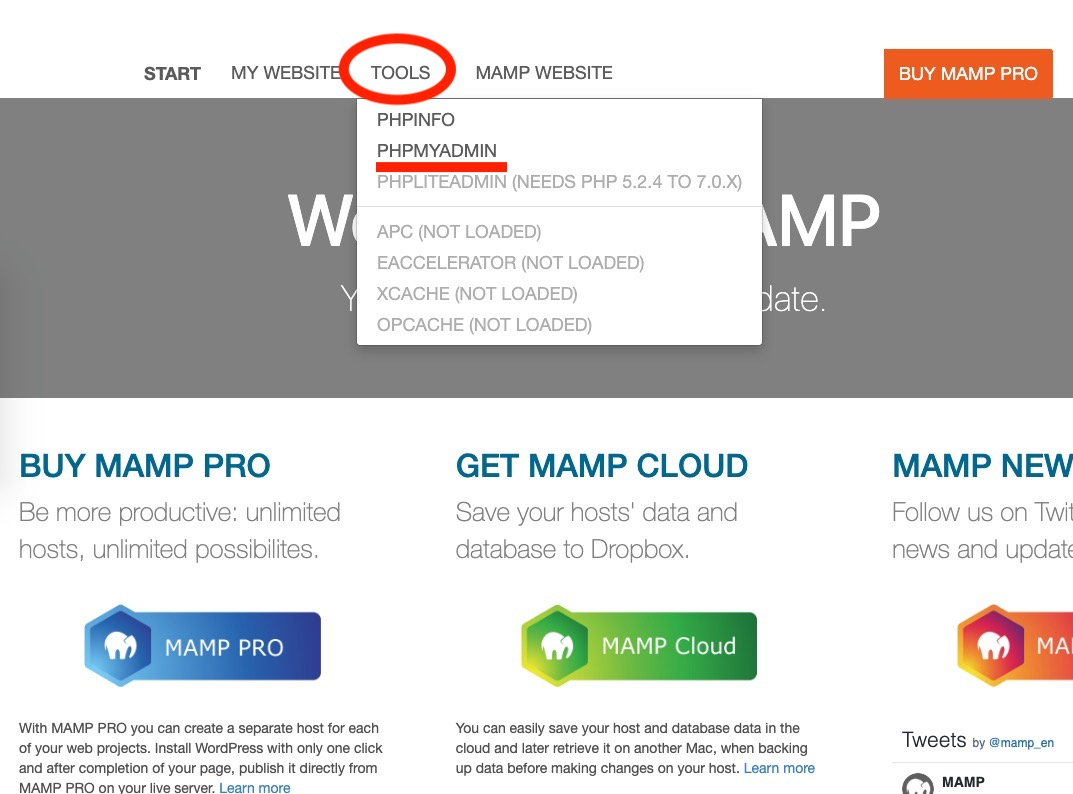
\includegraphics[width=0.7\textwidth]{Project_Document/phpmyadmin}
                        \caption{phpMyAdmin on MAMP}
                    \end{figure}

                \item Now, you need to open `phpMyAdmin' and create a database. (I named it drupal) 
        
                    \begin{figure}[!ht]
                           \centering
                           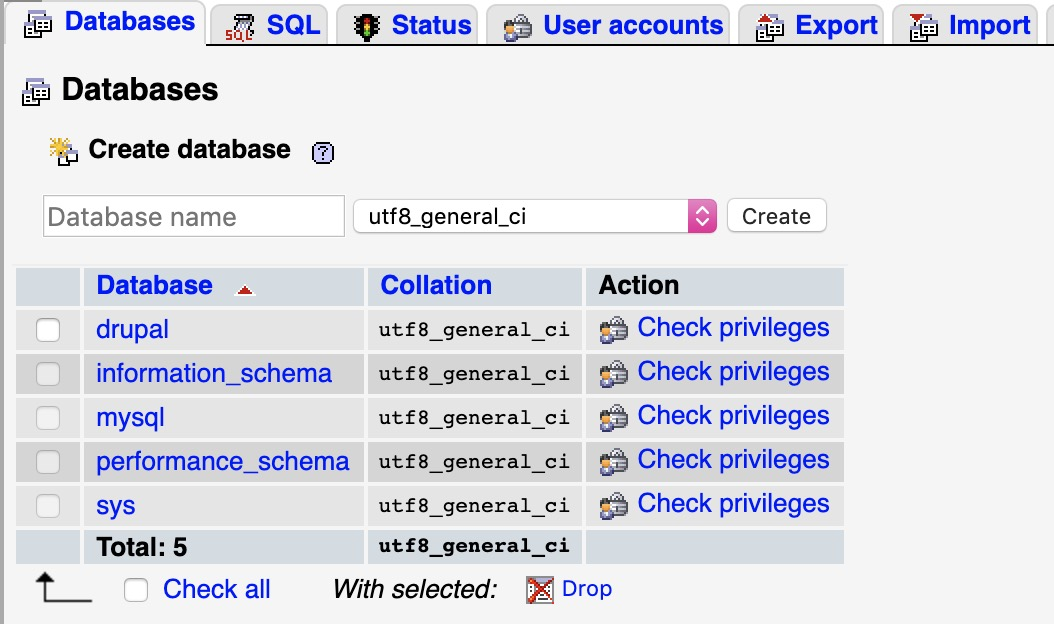
\includegraphics[width=0.7\textwidth]{Project_Document/1}
                        \caption{phpMyAdmin}
                    \end{figure}
\newpage                
                \item Then, click the database and go to `Import' tab at the top. (I marked in the red square) 
                
                    \begin{figure}[!ht]
                           \centering
                           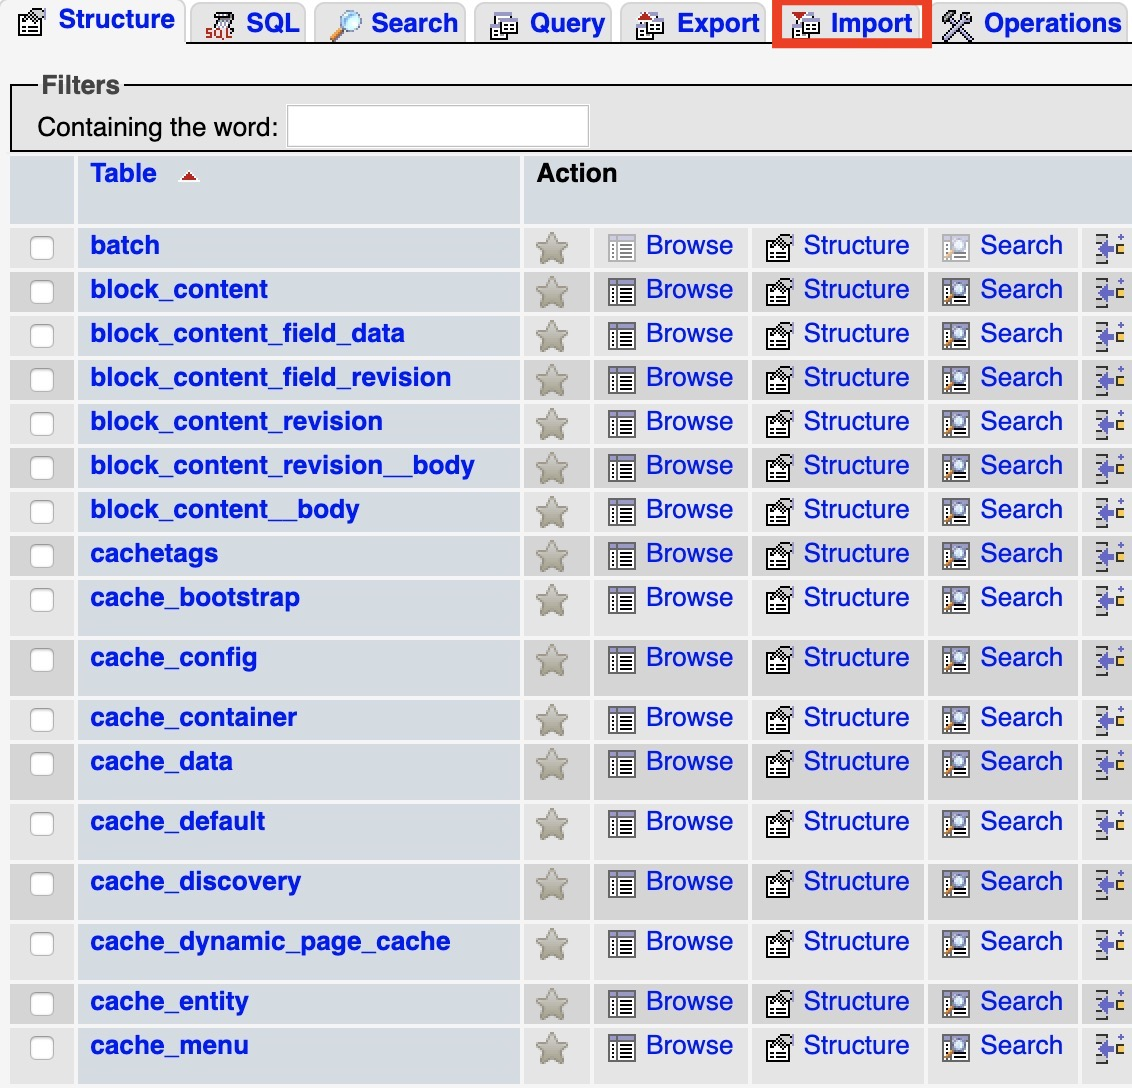
\includegraphics[width=0.7\textwidth]{Project_Document/2}
                        \caption{`Import' Button on phpMyAdmin }
                    \end{figure}
                
                \item Then, click the `choose the file' and open the file name `sqlbackup.sql.zip' in thie repo. Now, you have imported our back-up files from the server. \\
                Open this file by any test editor
                
\begin{lstlisting}[language=bash]
`html' or `any folder for your Drupal directory'/sites/default/settings.php
\end{lstlisting}
            
                Find this lines of the code (it is located at the very bottom) \\
               
                    \begin{figure}[!ht]
                           \centering
                           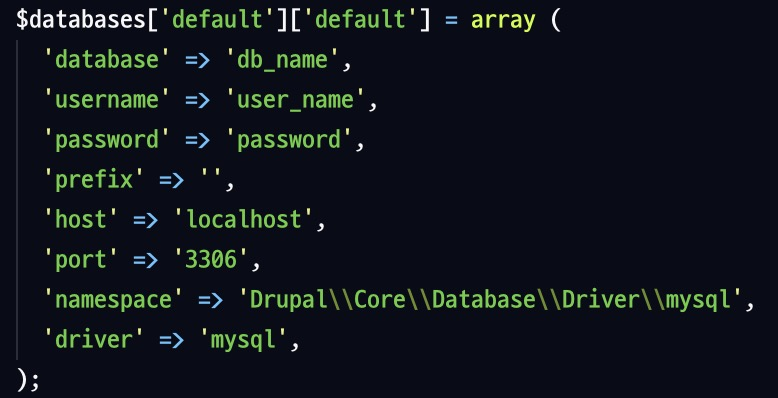
\includegraphics[width=0.5\textwidth]{Project_Document/codes}
                        \caption{Database Code}
                    \end{figure}
            
                Please change database, username and password sections to match your local settings (the database you have imported the above) Finally, you can connect our Drupal Website. If you are using MAMP, MAMP already sets the username and the password for MySQL for you. This is where you can find your username and password (in MAMP main page). All you needs are user and password. (Mostly, these are already set as root and root) 
           
                    \begin{figure}[!ht]
                           \centering
                           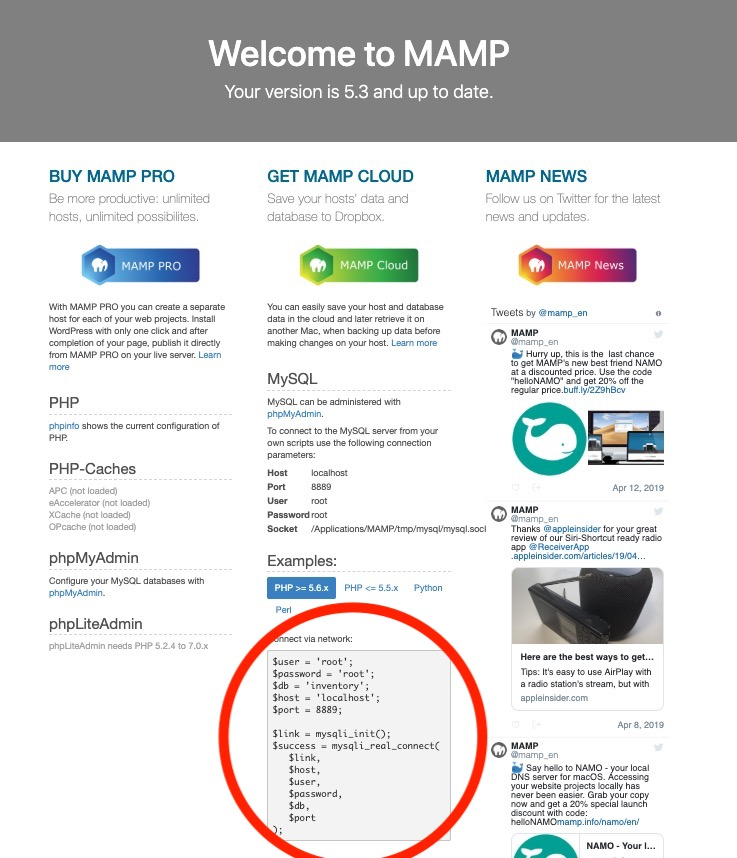
\includegraphics[width=0.5\textwidth]{Project_Document/sqlinfo}
                        \caption{Database Information on MAMP}
                    \end{figure}
                    
            \item You can connect to your localhost by:
            
\begin{lstlisting}[language=bash]
http://localhost or http://localhost:8888
\end{lstlisting}
            
            You may want to log in to the site to see how the site actually works. (Click `+' sign at the top right corner) 
            
                \begin{figure}[!ht]
                       \centering
                         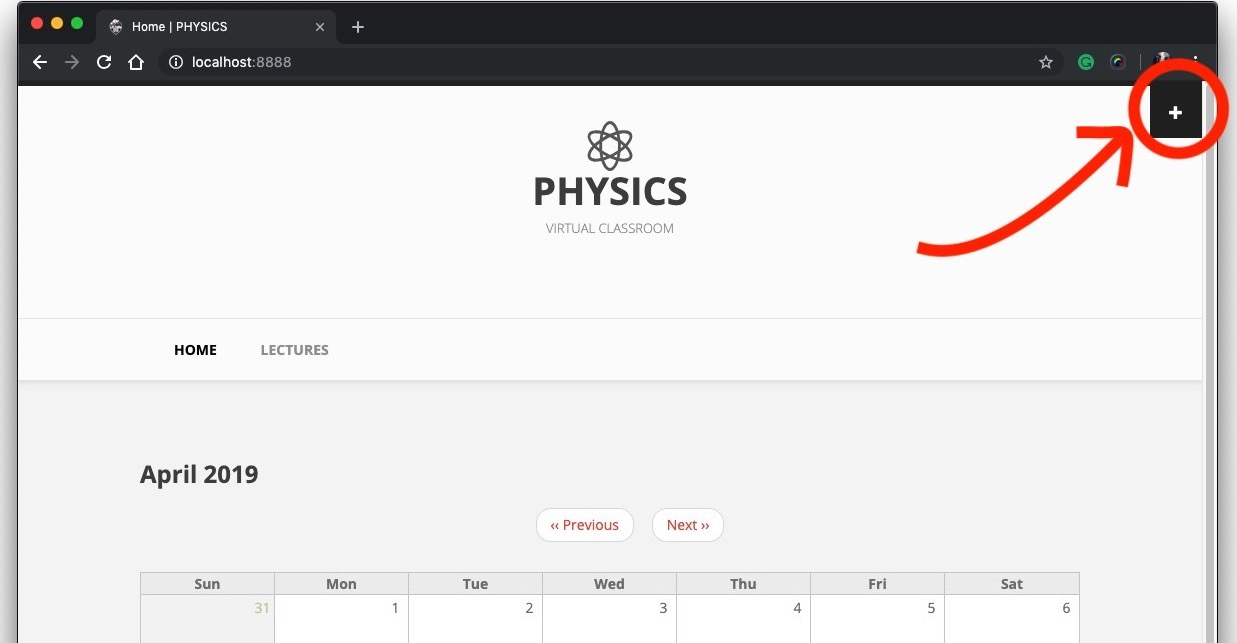
\includegraphics[width=0.6\textwidth]{Project_Document/login.jpg}
                    \caption{Login Button on Physic Virtual Classroom Website}
                \end{figure}
\newpage            
            If you don’t know the username and the password, please contact Walsh, Kenneth.
            
            Note: if you are trying to connect to Drupal, not by localhost, you need to modify this code in the same setting.php file. Add your host name in the array.
            
                \begin{figure}[!ht]
                       \centering
                       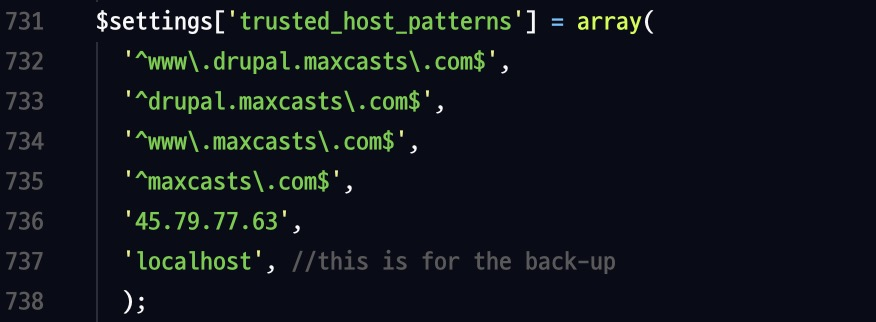
\includegraphics[width=0.7\textwidth]{Project_Document/host.jpg}
                    \caption{setting.php File}
                \end{figure}
        \end{enumerate}  
        
    \subsection{User manual}
        \subsubsection{Add Lecture}
            \begin{enumerate}
            	\item Log in to an administrator account. Only users who have an administration account can add lectures.
            	\item Click `Content' on the toolbar.
            	   \begin{figure}[!ht]
            	        \centering
                        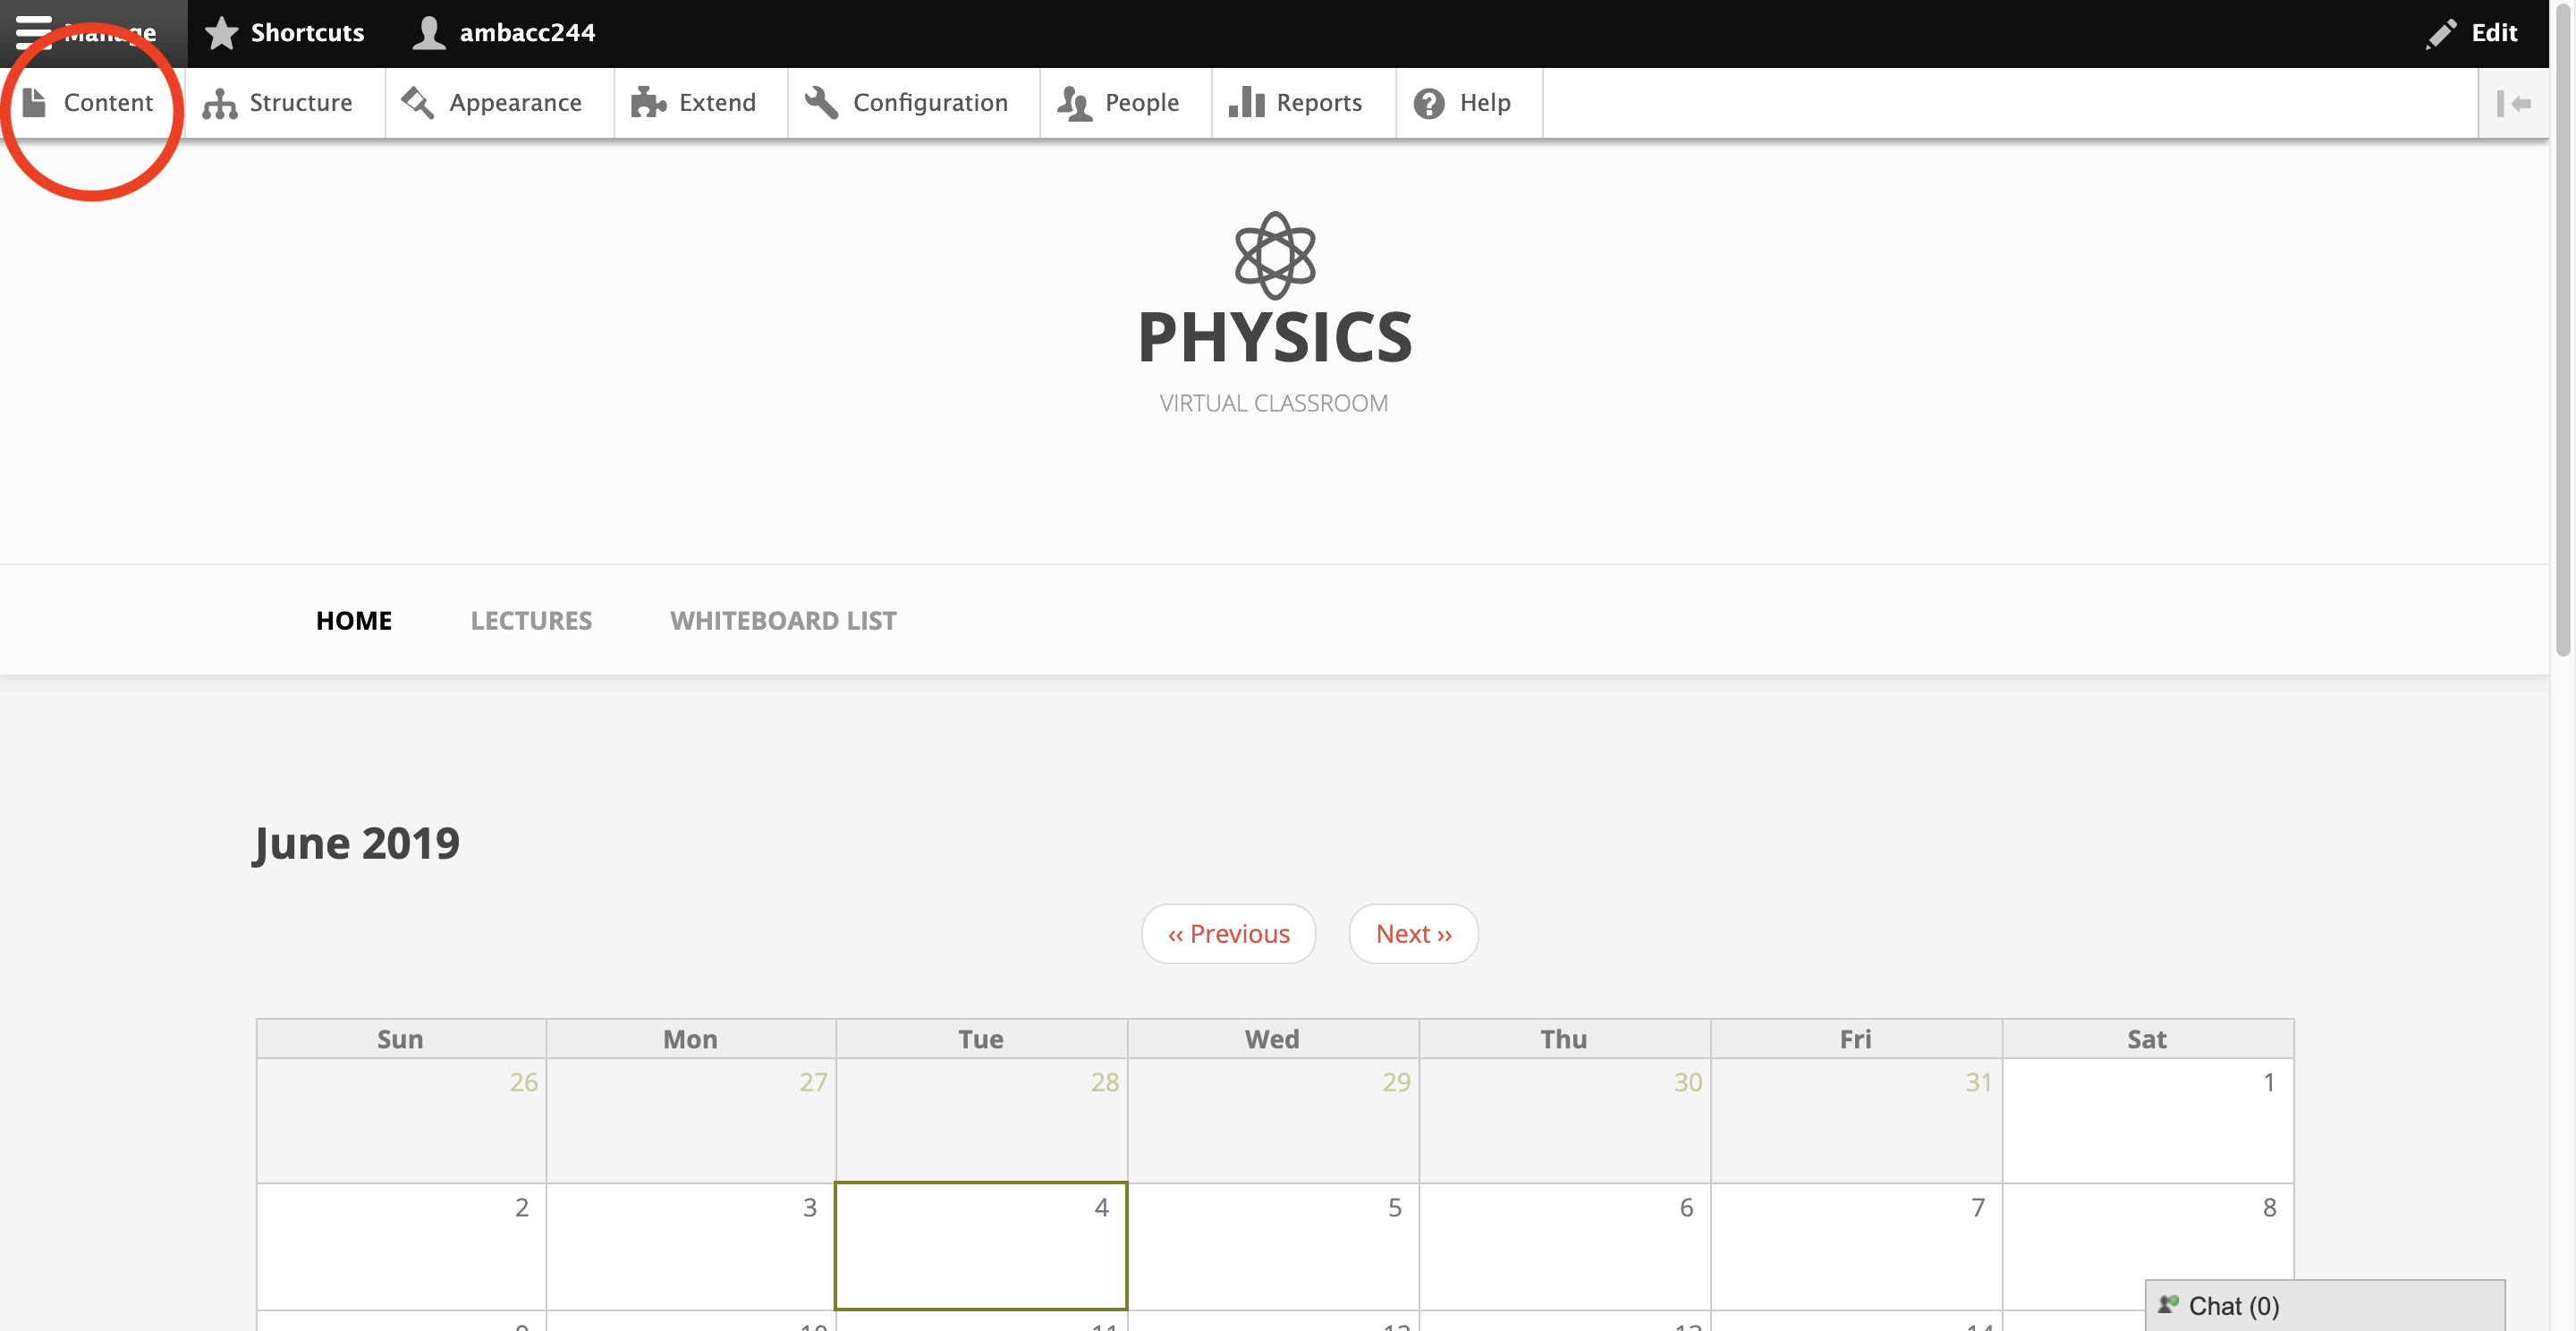
\includegraphics[width=0.7\textwidth]{Project_Document/content}
                        \caption{`Content' Button on the Physics Virtual Classroom Website}
                    \end{figure}
            	\item Click `+Add content' $\,\to\,$ `Lecture Video'
            	\item Need to fill out `Create Lecture Video' form. There are four parts to fill out which are title, body, date, and video 
            	    \begin{itemize}
                    	\item Title: title of the lecture
                    	\item Body: lecture description
                    	\item Data: lecture date and time
                    	\item Video: YouTube or YouTube live video link
                    \end{itemize} 
            	\item Click `Preview' to check lecture information again.
            	\item Click `Save' to add the lecture.
            \end{enumerate}
            
        \subsubsection{Edit or Delete Lecture}
            \begin{enumerate}
            	\item Log in to an administrator account. Only users who have an administration account can edit lectures.
         	
            	\item Click `LECTURES' on the toolbar.
            	    \begin{figure}[!ht]
            	        \centering
                        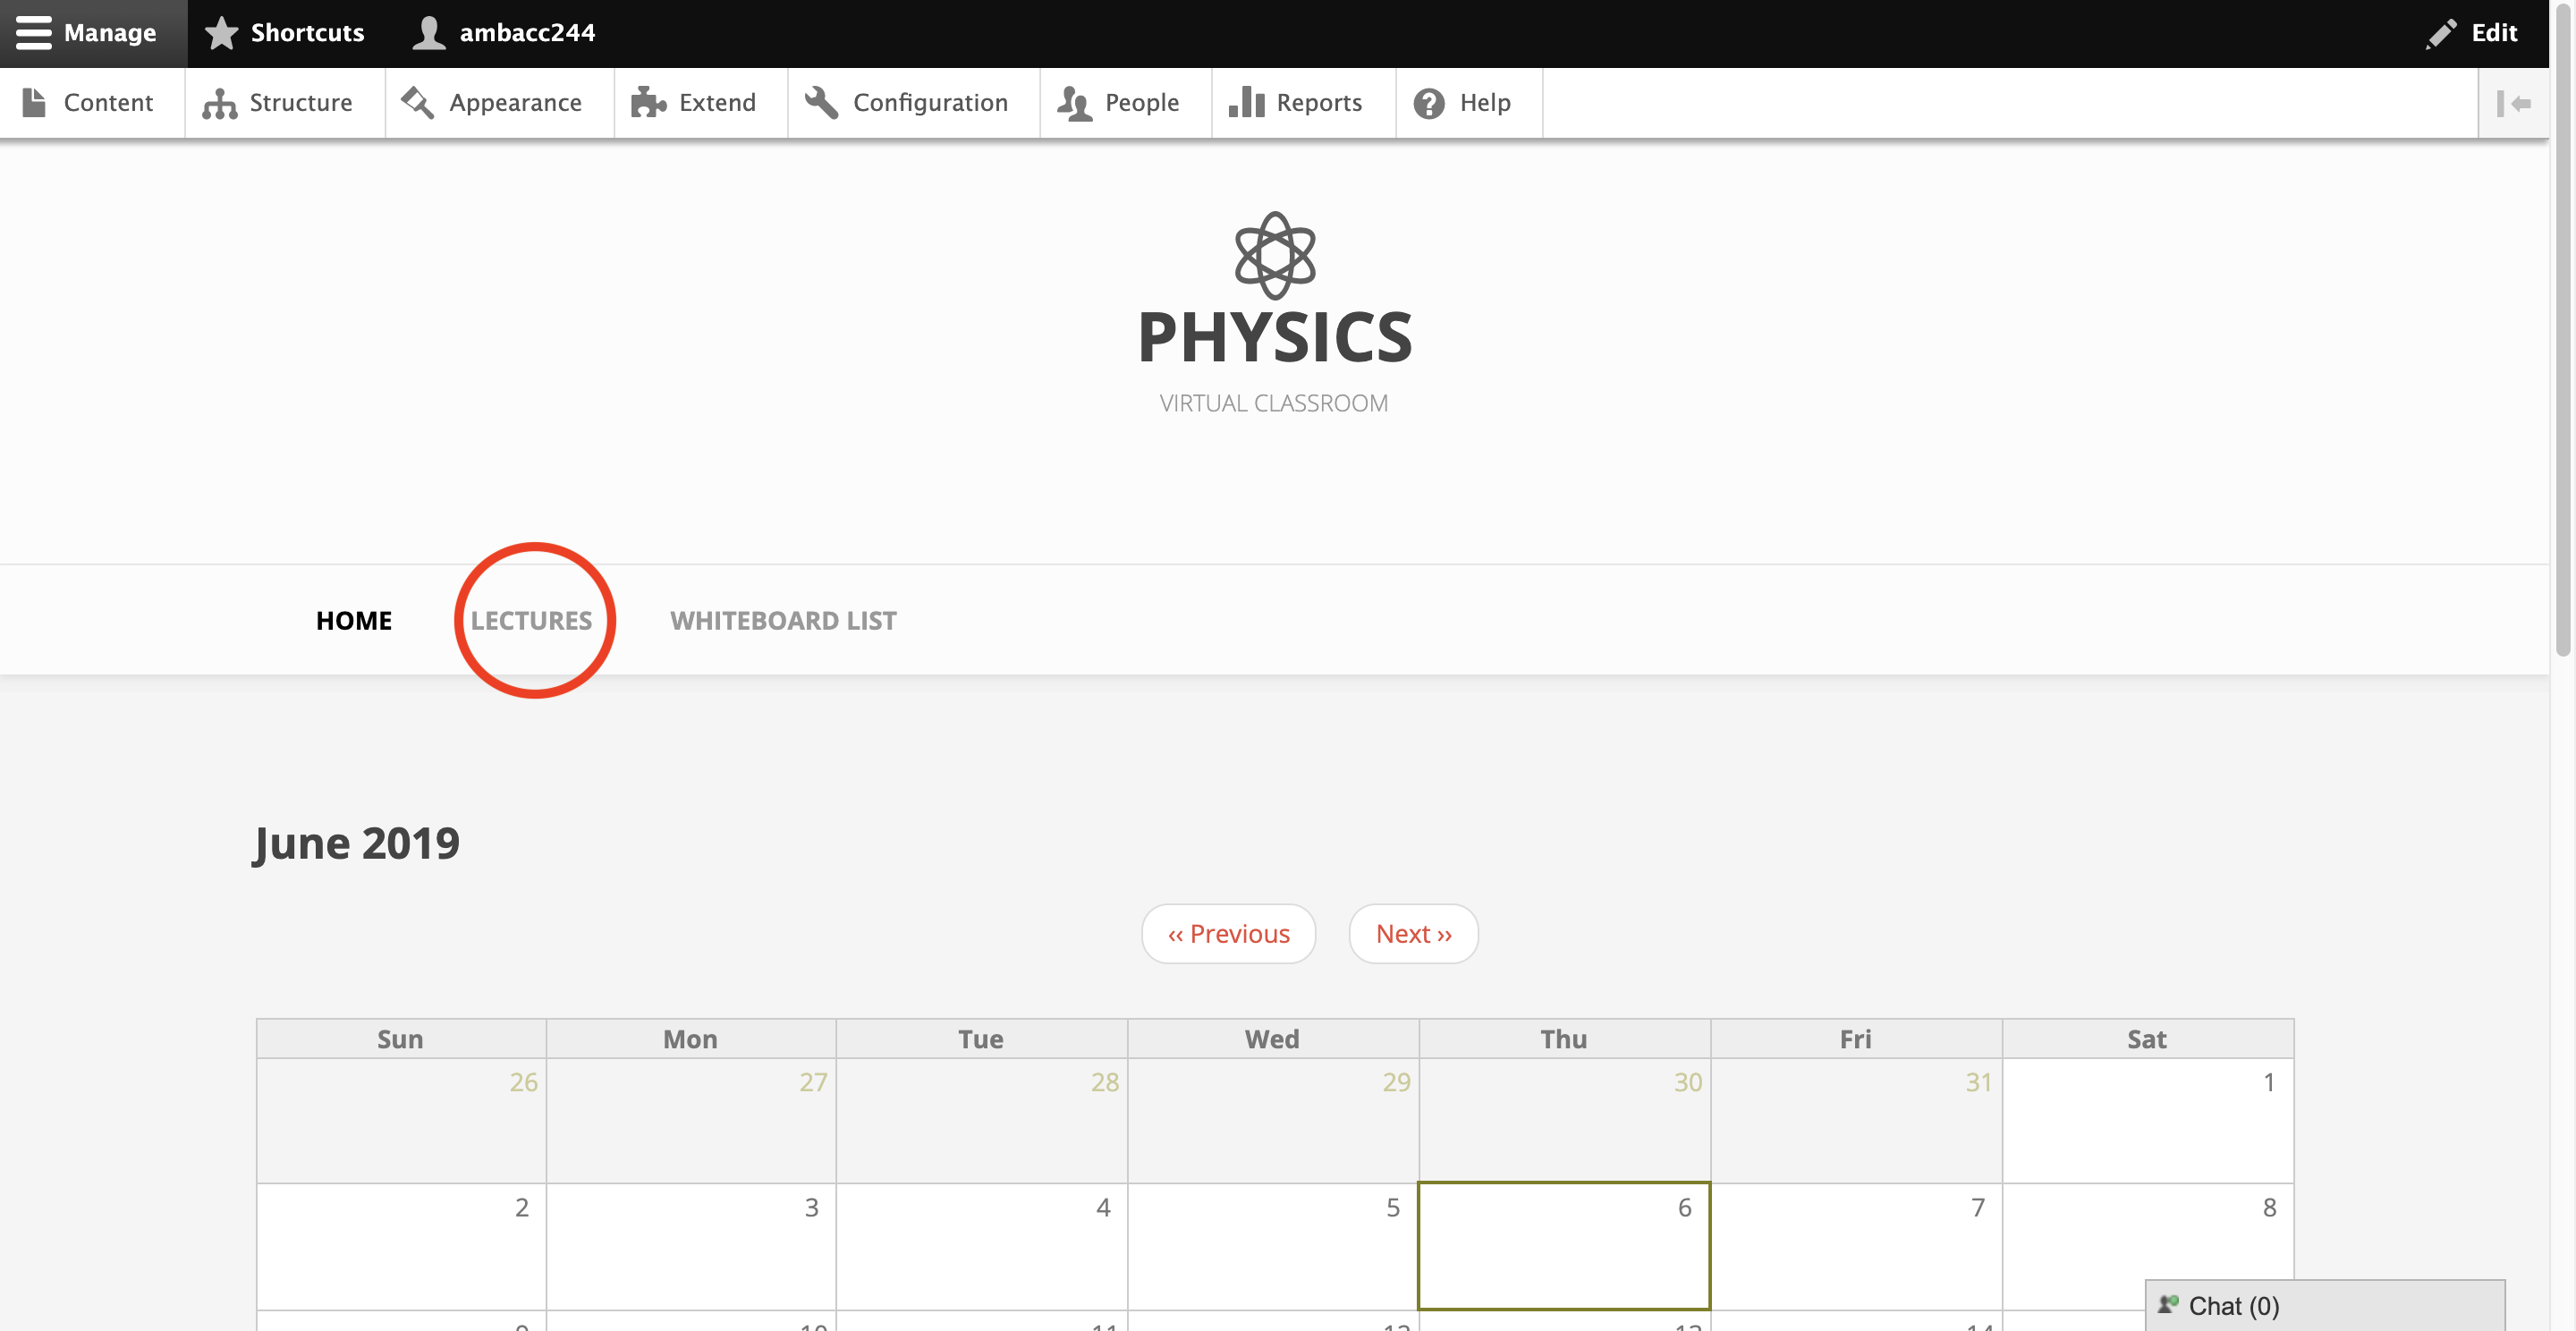
\includegraphics[width=0.7\textwidth]{Project_Document/lectures.png}
                        \caption{`LECTURES' Button on the Physics Virtual Classroom Website}
                    \end{figure}
            	\item Click the lecture which you want to edit or delete on the table.
            	\item Click `Edit' or `Delete' to edit or delete the lecture.
            \end{enumerate}
 
        \subsubsection{Add, Edit or Delete whiteboard on the whiteboard list}
            \begin{enumerate}
            	\item Log in to an administrator account. Only users who have an administration account can add lectures.
            	\item Click `WHITEBOARD LIST' on the toolbar.
            	    \begin{figure}[!ht]
            	        \centering
                        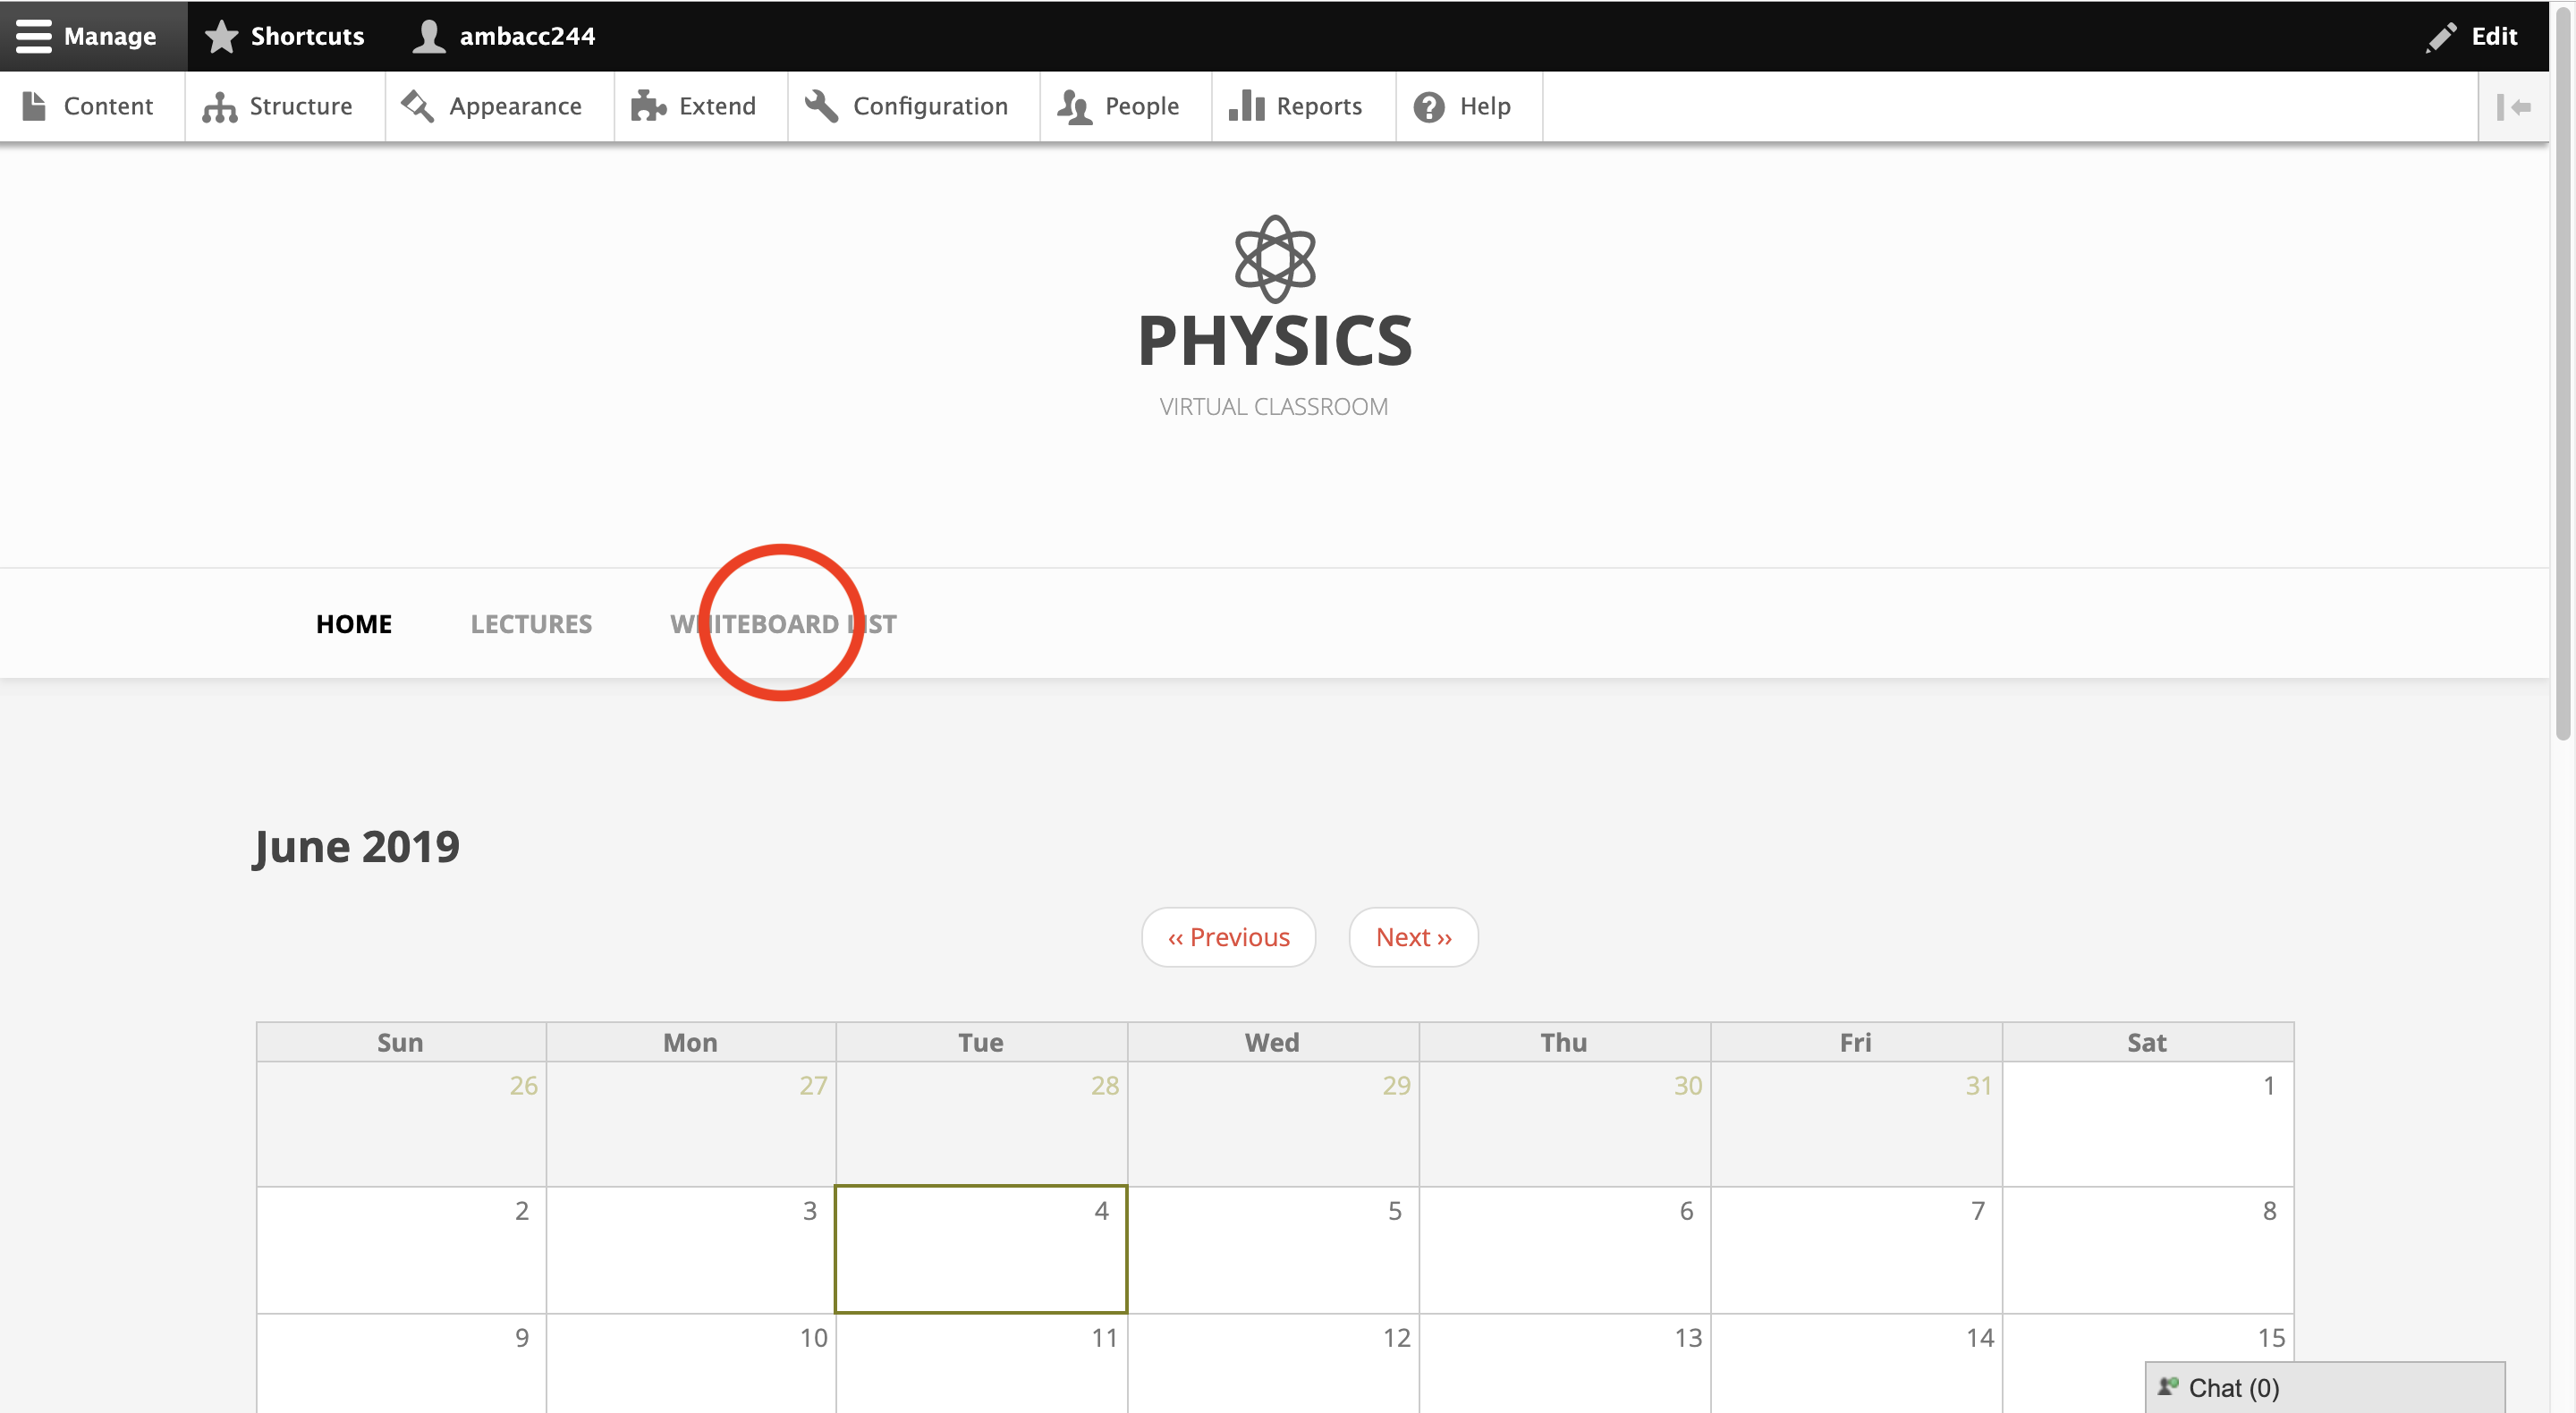
\includegraphics[width=0.7\textwidth]{Project_Document/whiteboard.png}
                        \caption{`WHITEBOARD LIST' Button on the Physics Virtual Classroom Website}
                    \end{figure}
\newpage                   
            	\item Click `Edit' $\,\to\,$ `Source' 
            	    \begin{figure}[!ht]
            	        \centering
                        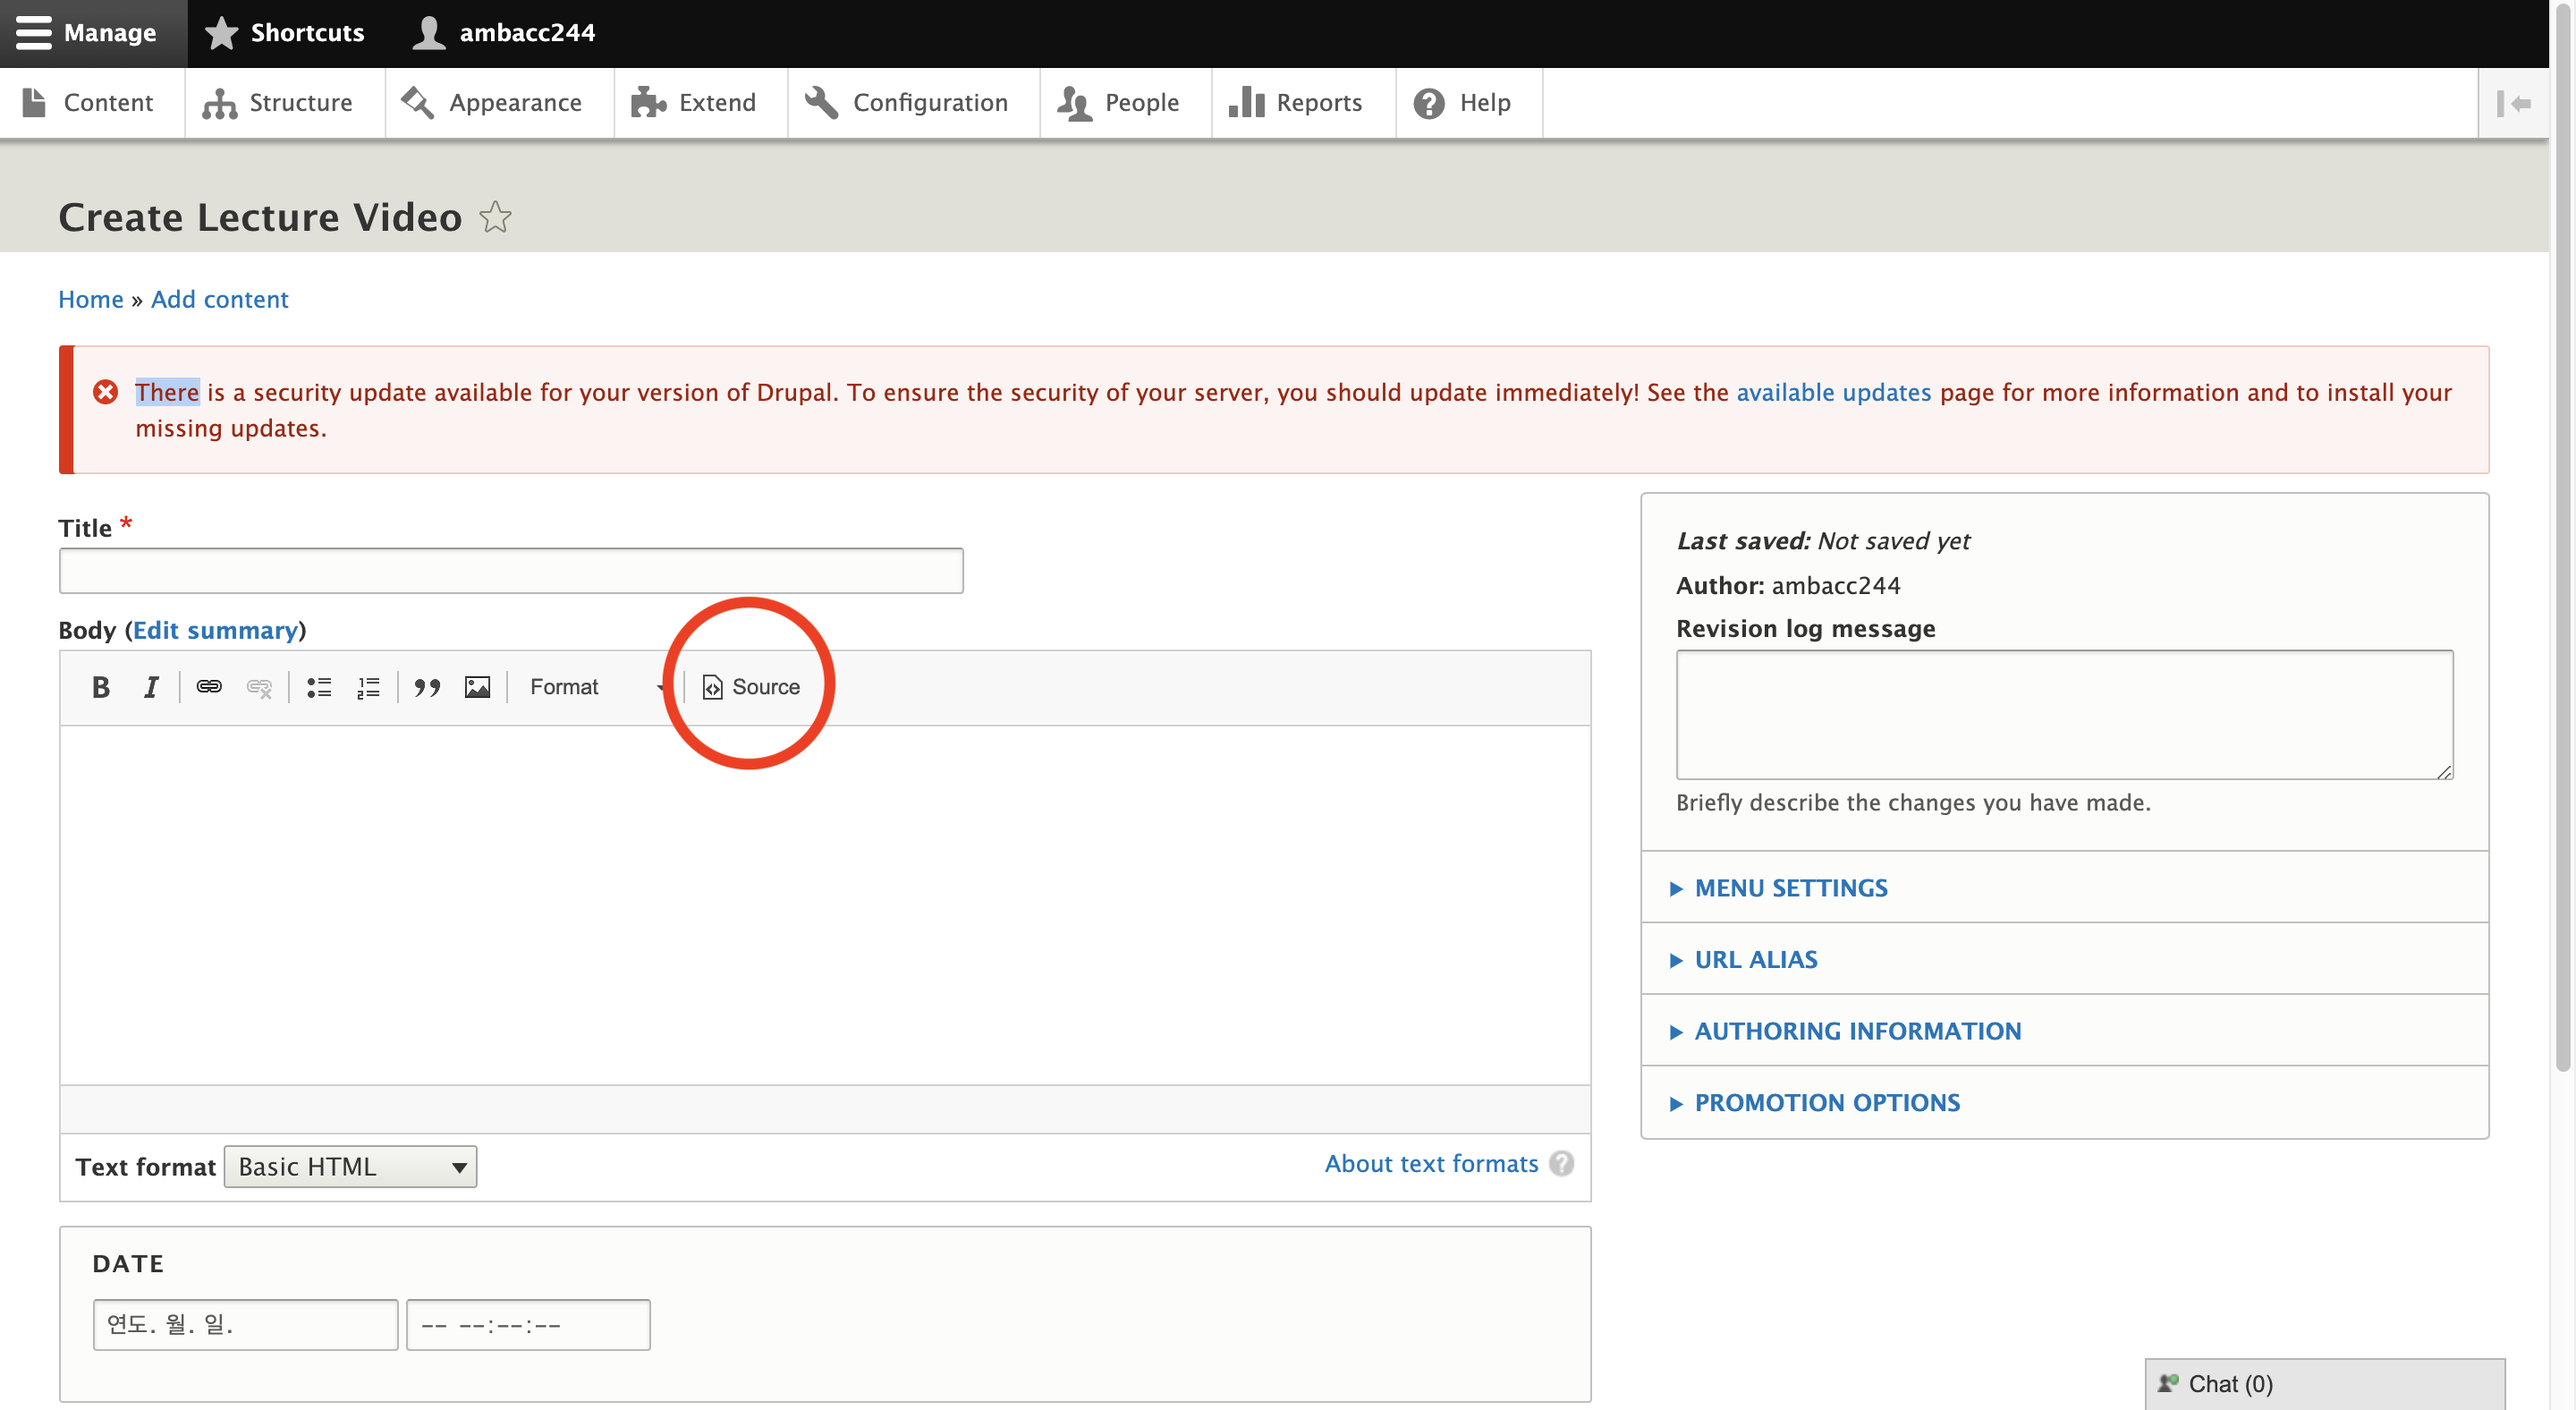
\includegraphics[width=0.7\textwidth]{Project_Document/source.png}
                        \caption{`Source' Button on the Physics Virtual Classroom Website}
                    \end{figure}
            	\item Change code to create and delete whiteboard buttons. 
            \end{enumerate}
        
        \subsubsection{Create new Administrator Account}
            \begin{enumerate}
                \item Click `People’ on the toolbar.
                    \begin{figure}[!ht]
            	        \centering
                        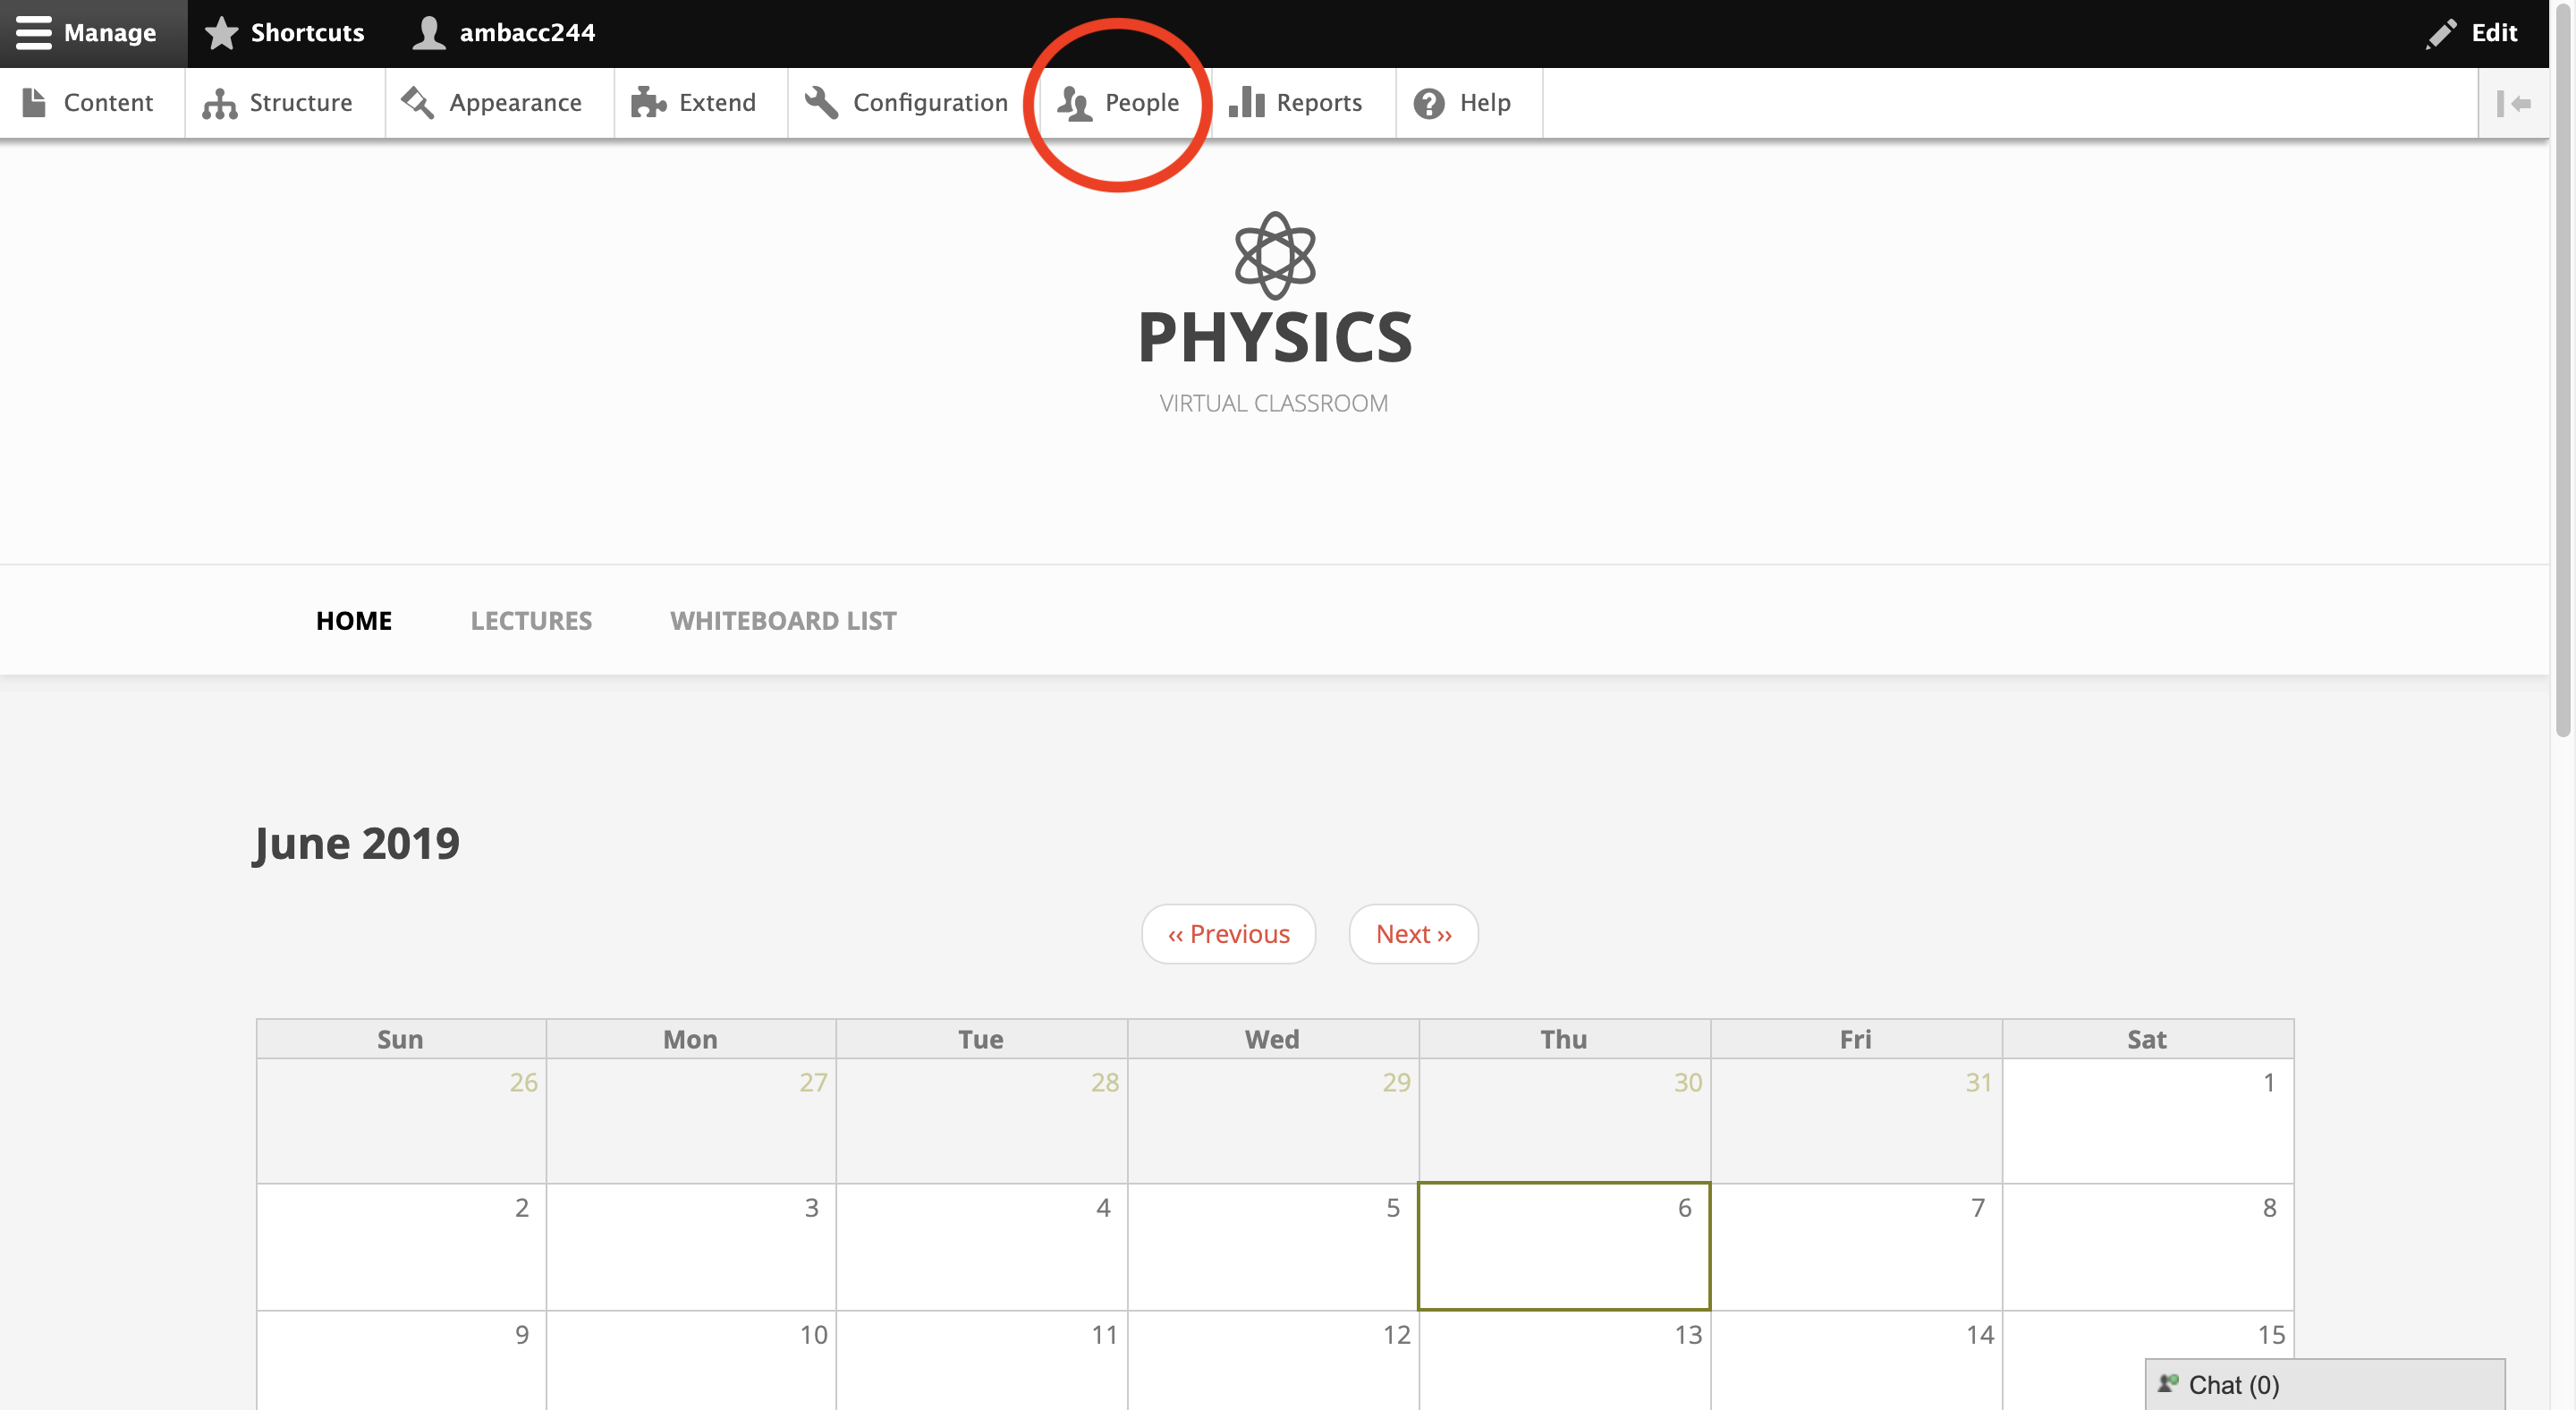
\includegraphics[width=0.7\textwidth]{Project_Document/people.png}
                        \caption{`People' Button on the Physics Virtual Classroom Website}
                    \end{figure}
                \item Click `+Add user'
                \item Need to fill out `Add user' form. 
                    \begin{itemize}
                        \item Email address: Optional
                        \item Username: Required
                        \item Password: Required
                        \item Status: Set as  `Active’
                        \item Roles: \textbf{Set as `Administrator'}
                        \item Picture: Optional
                    \end{itemize}
                \item Click `Create new account’	
            \end{enumerate}
            
    \subsection{Back-up Guide}        
        If you want to make back-ups of the current website, you need to duplicate the current folder of Drupal and export the current database. Then, follow the above instruction to install or re-install the website. Another easy tool for back-ups may be available as a module. You may want to find it at Drupal's module website.
    
    \subsection{Additional Information}    
        \begin{enumerate}  
            \item The website does not require any permission to read any contents on the website. If you want to fix this, you need to download a module that will block anonymous users to read the specific contents of the website.
            \item Drupal encourages users to keep the website up-to-date. Updating the website may cause some problems, so it’s always good to have the latest back-ups.
            \item Currently, the website is run on `http’, not `https’. Some browsers may show a warning message because of the security issue. This can be fixed within the server. You also may want to change some settings of Drupal.
            
            \item When you upload content, URL of the content may be ugly. It looks like this: drupal.org/node\#\#. So, you may want to change the URL of the content manually. The feature can be found where you can edit the content. (It’s called URL ALIAS) It looks better if you keep adding numbers of what you are posting. For example, /lecture1, /lecture2. There may some module that makes this automatic, but we could not find it.
            
            \item The whiteboards in the list of whiteboards are currently managed by Eric’s account on AWW. This whiteboard may be removed if the whiteboard hasn’t used for a long time. In case, you may want to create your own account on AWW and make the whiteboards. It will last a very long time (we haven’t checked how long those last).
            \item Drupal can be easily crushed if you make an inappropriate change. So, please test it on your local machine and apply it on the main server.
        \end{enumerate}
\clearpage 
\end{document}
